% !TeX program = xelatex
\documentclass[a4paper,10pt]{article}

% ============================================================================
% កញ្ចប់បណ្ណាល័យ (Packages) – តាមលំនាំស្តង់ដារ អនុវិទ្យាល័យព្រះក្រសាំង (ls_plan.tex)
% បរិបទ៖ ថ្នាក់រៀនគ្មានស្លាយ LCD – បង្រៀនដោយប្រើក្ដារខៀន និងសន្លឹកកិច្ចការសិស្សស-ខ្មៅជាគោល
% ============================================================================
\usepackage[a4paper, left=0.95cm, right=0.95cm, top=0.85cm, bottom=0.92cm, footskip=0.52cm]{geometry}
\usepackage{amsmath}
\usepackage{unicode-math}
\usepackage{fontspec}
\usepackage{array, longtable, multirow, colortbl}
\usepackage[table]{xcolor}
\usepackage{enumitem}
\usepackage{pifont}
\usepackage{fancyhdr}
\usepackage{tikz}
\usetikzlibrary{calc, arrows.meta, angles, quotes, decorations.markings, positioning, babel}

\makeatletter
\let\@expl@@@mark@update@singlecol@structures@@\relax
\makeatother

% ============================================================================
% ការកំណត់ពុម្ពអក្សរផ្លូវការ (Cross-Platform Fonts Configuration)
% ============================================================================
\providecommand{\NGSFindFonts}{%
  \IfFileExists{C:/Windows/Fonts/cambria.ttc}{%
    \def\NGSSysPath{C:/Windows/Fonts/}%
    \def\NGSUserPath{C:/Users/KIT/AppData/Local/Microsoft/Windows/Fonts/}%
  }{%
    \IfFileExists{./fonts/KhmerOSsiemreap.ttf}{\def\NGSSysPath{./fonts/}\def\NGSUserPath{./fonts/}}{%
    \IfFileExists{../fonts/KhmerOSsiemreap.ttf}{\def\NGSSysPath{../fonts/}\def\NGSUserPath{../fonts/}}{%
    \IfFileExists{../../fonts/KhmerOSsiemreap.ttf}{\def\NGSSysPath{../../fonts/}\def\NGSUserPath{../../fonts/}}{%
    \IfFileExists{../../../fonts/KhmerOSsiemreap.ttf}{\def\NGSSysPath{../../../fonts/}\def\NGSUserPath{../../../fonts/}}{%
    \IfFileExists{../../../../fonts/KhmerOSsiemreap.ttf}{\def\NGSSysPath{../../../../fonts/}\def\NGSUserPath{../../../../fonts/}}{%
    \IfFileExists{../../../../../fonts/KhmerOSsiemreap.ttf}{\def\NGSSysPath{../../../../../fonts/}\def\NGSUserPath{../../../../../fonts/}}{%
    \IfFileExists{../../../../../../fonts/KhmerOSsiemreap.ttf}{\def\NGSSysPath{../../../../../../fonts/}\def\NGSUserPath{../../../../../../fonts/}}{%
      \def\NGSSysPath{../../../../../../../fonts/}\def\NGSUserPath{../../../../../../../fonts/}%
    }}}}}}}%
  }%
}
\NGSFindFonts

\setmathfont[Path={\NGSSysPath}, FontIndex=1, Scale=1.02]{cambria.ttc}
\defaultfontfeatures{Ligatures=TeX}

\setmainfont[
  Path={\NGSUserPath},
  Extension=.ttf,
  Script=Khmer,
  BoldFont={KhmerOSsiemreap},
  BoldFeatures={FakeBold=1.8},
  ItalicFont={KhmerOSsiemreap},
  ItalicFeatures={FakeSlant=0.25},
  BoldItalicFont={KhmerOSsiemreap},
  BoldItalicFeatures={FakeBold=1.8, FakeSlant=0.25}
]{KhmerOSsiemreap}

\newfontfamily\muol[Path={\NGSUserPath}, Extension=.ttf, Script=Khmer]{KhmerOSmuollight}
\newfontfamily\TimesEn[Path={\NGSSysPath}, Extension=.ttf, BoldFont={timesbd}, ItalicFont={timesi}, BoldItalicFont={timesbi}]{times}
\newfontfamily\NagaBold[Path={\NGSUserPath}, Extension=.ttf]{AKbalthom Naga Bold}
\newfontfamily\CalibriFont[Path={\NGSSysPath}, Extension=.ttf]{calibri}
\newfontfamily\Tacteing[Path={\NGSUserPath}]{TACTENG.TTF}
\newfontfamily\CourierBullet[Path={\NGSSysPath}, Extension=.ttf]{cour}
\newcommand{\wcirc}{{\CourierBullet\fontsize{9.5pt}{11pt}\selectfont o}}

\XeTeXlinebreaklocale "km"
\XeTeXlinebreakskip = 0pt plus 1pt minus 0.1pt

\definecolor{stepgray}{HTML}{D9D9D9}
\definecolor{headgray}{HTML}{F2F2F2}
\definecolor{boxgray}{HTML}{D9D9D9}
\definecolor{darkred}{HTML}{C00000}
\definecolor{red5e}{HTML}{FF0000}

\pagestyle{fancy}
\fancyhf{}
\renewcommand{\headrulewidth}{0pt}
\fancyfoot[R]{\CalibriFont\fontsize{11pt}{13pt}\selectfont\thepage}

\setlength{\parindent}{0pt}
\setlength{\parskip}{0pt}
\setlength{\tabcolsep}{3.8pt}

\newcolumntype{L}[1]{>{\raggedright\arraybackslash}p{#1}}

\newcommand{\en}[1]{{\TimesEn #1}}
\newcommand{\enbf}[1]{{\TimesEn\textbf{#1}}}
\newcommand{\unit}[1]{\,\text{\en{#1}}}
\newcommand{\fiveE}[1]{{\NagaBold\fontsize{9.5pt}{13pt}\selectfont\textcolor{red5e}{#1}}}
\newcommand{\timenote}[1]{\textcolor{darkred}{\textit{#1}}}
\newcommand{\redsub}[1]{\textcolor{darkred}{#1}}
\newcommand{\graybox}[1]{\colorbox{boxgray}{\strut\hspace{2pt}#1\hspace{2pt}}}
\newcommand{\ditem}{\tikz[baseline=-0.5ex]\fill (0,0.42ex) -- (0.42ex,0) -- (0,-0.42ex) -- (-0.42ex,0) -- cycle;\hspace{0.3em}}
\newcommand{\cnum}[1]{{\fontsize{10.5pt}{12pt}\selectfont\ding{\numexpr171+#1\relax}}\hspace{0.2em}}
\newcommand{\cfig}[1]{\par\vspace{4pt}{\centering #1\par}\vspace{4pt}}
\newcommand{\stepheader}[1]{\multicolumn{3}{|c|}{\cellcolor{stepgray}\muol #1} \\* \noalign{\hrule height 0.4pt}}
\newcommand{\tri}[1]{\ensuremath{\triangle #1}}
\newcommand{\ang}[1]{\ensuremath{\angle #1}}
\newcommand{\cg}{\ensuremath{\cong}}
\newcommand{\khmflourish}{{\Tacteing\fontsize{36pt}{14pt}\selectfont\raisebox{-5pt}{3}}}

\tikzset{
  tk1/.style={postaction={decorate},decoration={markings,mark=at position 0.50 with {\draw[black, line width=0.85pt](0,-0.095)--(0,0.095);}}},
  tk2/.style={postaction={decorate},decoration={markings,
    mark=at position 0.45 with {\draw[black, line width=0.85pt](0,-0.095)--(0,0.095);},
    mark=at position 0.55 with {\draw[black, line width=0.85pt](0,-0.095)--(0,0.095);}}},
  tk3/.style={postaction={decorate},decoration={markings,
    mark=at position 0.42 with {\draw[black, line width=0.85pt](0,-0.095)--(0,0.095);},
    mark=at position 0.50 with {\draw[black, line width=0.85pt](0,-0.095)--(0,0.095);},
    mark=at position 0.58 with {\draw[black, line width=0.85pt](0,-0.095)--(0,0.095);}}},
  par1/.style={postaction={decorate},decoration={markings,mark=at position 0.52 with {\draw[black, line width=0.85pt](-0.07,0.08)--(0.05,0)--(-0.07,-0.08);}}},
  par2/.style={postaction={decorate},decoration={markings,
    mark=at position 0.46 with {\draw[black, line width=0.85pt](-0.07,0.08)--(0.05,0)--(-0.07,-0.08);},
    mark=at position 0.58 with {\draw[black, line width=0.85pt](-0.07,0.08)--(0.05,0)--(-0.07,-0.08);}}}
}

% ============================================================================
% ម៉ាក្រូរូបភាពធរណីមាត្រស-ខ្មៅ (Proportional 4.0–7.2 cm B&W TikZ Diagrams)
% ============================================================================

% ១. រំលឹកមេរៀនទាក់ទង៖ មុំឆ្លាស់ក្នុង/មុំក្នុងរួមខាង + លក្ខណៈ ម-ជ-ម
\newcommand{\figPrereqPARA}{%
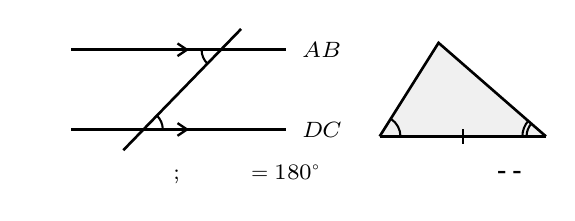
\begin{tikzpicture}[scale=0.88, every node/.style={font=\footnotesize, text=black}]
  % ឆ្វេង៖ បន្ទាត់ស្រប មុំឆ្លាស់ក្នុង និងមុំក្នុងរួមខាង
  \begin{scope}[shift={(0,0)}]
    \draw[black, line width=0.95pt, par1] (0,1.35) -- (3.1,1.35) node[right=2pt] {$AB$};
    \draw[black, line width=0.95pt, par1] (0,0.20) -- (3.1,0.20) node[right=2pt] {$DC$};
    \draw[black, line width=0.95pt] (2.45,1.65) -- (0.75,-0.10);
    \draw[black, line width=0.75pt] ($(2.16,1.35)+(180:0.28)$) arc (180:226:0.28);
    \draw[black, line width=0.75pt] ($(1.04,0.20)+(0:0.28)$) arc (0:46:0.28);
    \node at (1.55,-0.45) {មុំឆ្លាស់ក្នុងស្មើគ្នា; មុំរួមខាង $=180^\circ$};
  \end{scope}
  % ស្ដាំ៖ ត្រីកោណប៉ុនគ្នា ម-ជ-ម
  \begin{scope}[shift={(4.45,0.10)}]
    \coordinate (P) at (0,0); \coordinate (Q) at (2.4,0); \coordinate (R) at (0.85,1.35);
    \fill[gray!12] (P)--(Q)--(R)--cycle;
    \draw[black, line width=0.95pt, tk1] (P)--(Q);
    \draw[black, line width=0.95pt] (Q)--(R)--(P);
    \draw[black, line width=0.75pt] ($(P)+(0:0.30)$) arc (0:56:0.30);
    \draw[black, line width=0.75pt] ($(Q)+(180:0.28)$) arc (180:138:0.28);
    \draw[black, line width=0.75pt] ($(Q)+(180:0.34)$) arc (180:138:0.34);
    \node at (1.20,-0.55) {លក្ខណៈប៉ុនគ្នា \textbf{ម-ជ-ម}};
  \end{scope}
\end{tikzpicture}}

% ២. E1 Engage: ជន្ទល់កន្ត្រៃលើកទំនិញរាងប្រលេឡូក្រាម ABCD
\newcommand{\figEngagePARA}{%
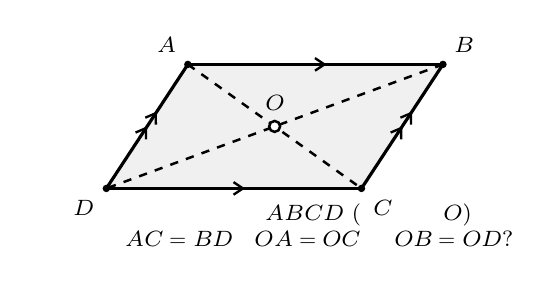
\begin{tikzpicture}[scale=0.90, every node/.style={font=\footnotesize, text=black}]
  \coordinate (D) at (0,0);
  \coordinate (C) at (3.60,0);
  \coordinate (A) at (1.15,1.75);
  \coordinate (B) at (4.75,1.75);
  \coordinate (O) at ($(A)!0.5!(C)$);
  \fill[gray!12] (A)--(B)--(C)--(D)--cycle;
  \draw[black, line width=1.15pt, par1] (A)--(B);
  \draw[black, line width=1.15pt, par1] (D)--(C);
  \draw[black, line width=1.15pt, par2] (D)--(A);
  \draw[black, line width=1.15pt, par2] (C)--(B);
  \draw[black, line width=0.9pt, dashed] (A)--(C) (B)--(D);
  \fill[black] (A) circle (1.5pt) node[above left=1pt] {$A$};
  \fill[black] (B) circle (1.5pt) node[above right=1pt] {$B$};
  \fill[black] (C) circle (1.5pt) node[below right=1pt] {$C$};
  \fill[black] (D) circle (1.5pt) node[below left=1pt] {$D$};
  \fill[white] (O) circle (2.2pt);
  \draw[black, line width=0.9pt] (O) circle (2.2pt);
  \node[above=2pt] at (O) {$O$};
  \node[align=center] at (2.38,-0.52) {ស៊ុមជន្ទល់កន្ត្រៃប្រលេឡូក្រាម $ABCD$ (ប៊ូឡុងកណ្ដាល $O$)\\តើអង្កត់ទ្រូង $AC = BD$ ឬ $OA=OC$ និង $OB=OD$?};
\end{tikzpicture}}

% ៣. E2/E3: រូបសំយោគទ្រឹស្ដីបទទី១–២ (អង្កត់ទ្រូង AC) និងទ្រឹស្ដីបទទី៣ (អង្កត់ទ្រូងពីរកាត់គ្នាត្រង់ O)
\newcommand{\figTheoremsPARA}{%
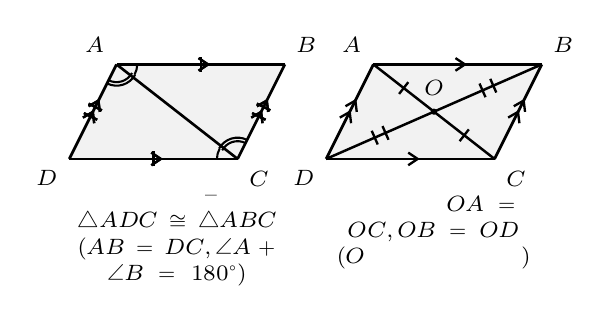
\begin{tikzpicture}[scale=0.75, every node/.style={font=\footnotesize, text=black}]
  % ឆ្វេង៖ ទ្រឹស្ដីបទទី១ និងទី២ (តាមសៀវភៅគោល ទំ.១៧០)
  \begin{scope}[shift={(0,0)}]
    \coordinate (D) at (0,0);
    \coordinate (C) at (2.85,0);
    \coordinate (A) at (0.80,1.60);
    \coordinate (B) at (3.65,1.60);
    \fill[gray!10] (A)--(B)--(C)--(D)--cycle;
    \draw[black, line width=1.0pt, par1, tk1] (A)--(B);
    \draw[black, line width=1.0pt, par1, tk1] (D)--(C);
    \draw[black, line width=1.0pt, par2, tk2] (D)--(A);
    \draw[black, line width=1.0pt, par2, tk2] (C)--(B);
    \draw[black, line width=0.95pt] (A)--(C);
    % មុំឆ្លាស់ក្នុង 1 & 2
    \draw[black, line width=0.75pt] ($(A)+(-29:0.35)$) arc (-29:0:0.35);
    \draw[black, line width=0.75pt] ($(C)+(151:0.35)$) arc (151:180:0.35);
    \draw[black, line width=0.75pt] ($(A)+(-117:0.30)$) arc (-117:-29:0.30);
    \draw[black, line width=0.75pt] ($(A)+(-117:0.36)$) arc (-117:-29:0.36);
    \draw[black, line width=0.75pt] ($(C)+(63:0.30)$) arc (63:151:0.30);
    \draw[black, line width=0.75pt] ($(C)+(63:0.36)$) arc (63:151:0.36);
    \node[above left=1pt] at (A) {$A$};
    \node[above right=1pt] at (B) {$B$};
    \node[below right=1pt] at (C) {$C$};
    \node[below left=1pt] at (D) {$D$};
    \node[anchor=north, text width=3.45cm, align=center] at (1.82,-0.45) {ទ្រឹស្ដីបទទី១--២៖ $\tri{ADC}\cg\tri{ABC}$\\($AB=DC, \ang{A}+\ang{B}=180^\circ$)};
  \end{scope}

  % ស្ដាំ៖ ទ្រឹស្ដីបទទី៣ (អង្កត់ទ្រូងកាត់គ្នាត្រង់ចំណុចកណ្ដាល O ទំ.១៧១)
  \begin{scope}[shift={(4.35,0)}]
    \coordinate (D) at (0,0);
    \coordinate (C) at (2.85,0);
    \coordinate (A) at (0.80,1.60);
    \coordinate (B) at (3.65,1.60);
    \coordinate (O) at ($(A)!0.5!(C)$);
    \fill[gray!10] (A)--(B)--(C)--(D)--cycle;
    \draw[black, line width=1.0pt, par1] (A)--(B);
    \draw[black, line width=1.0pt, par1] (D)--(C);
    \draw[black, line width=1.0pt, par2] (D)--(A);
    \draw[black, line width=1.0pt, par2] (C)--(B);
    \draw[black, line width=0.9pt, tk1] (A)--(O);
    \draw[black, line width=0.9pt, tk1] (O)--(C);
    \draw[black, line width=0.9pt, tk2] (B)--(O);
    \draw[black, line width=0.9pt, tk2] (O)--(D);
    \fill[black] (O) circle (1.5pt) node[above=2pt] {$O$};
    \node[above left=1pt] at (A) {$A$};
    \node[above right=1pt] at (B) {$B$};
    \node[below right=1pt] at (C) {$C$};
    \node[below left=1pt] at (D) {$D$};
    \node[anchor=north, text width=3.45cm, align=center] at (1.82,-0.45) {ទ្រឹស្ដីបទទី៣៖ $OA=OC, OB=OD$\\($O$ ជាផ្ចិតឆ្លុះប្រលេឡូក្រាម)};
  \end{scope}
\end{tikzpicture}}

% ៤. E4 Elaborate: លំហាត់គំរូទី១ (លំហាត់ទី៤ ទំ.១៨៥) & លំហាត់គំរូទី២ (លំហាត់ទី២ ទំ.១៨៥)
\newcommand{\figModelPARA}{%
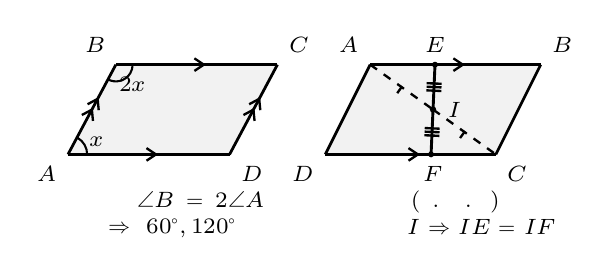
\begin{tikzpicture}[scale=0.76, every node/.style={font=\footnotesize, text=black}]
  % ឆ្វេង៖ លំហាត់ទី៤ ទំ.១៨៥ (\angle B = 2\angle A)
  \begin{scope}[shift={(0,0)}]
    \coordinate (A) at (0,0);
    \coordinate (D) at (2.70,0);
    \coordinate (B) at (0.80,1.50);
    \coordinate (C) at (3.50,1.50);
    \fill[gray!10] (A)--(B)--(C)--(D)--cycle;
    \draw[black, line width=1.0pt, par1] (B)--(C);
    \draw[black, line width=1.0pt, par1] (A)--(D);
    \draw[black, line width=1.0pt, par2] (A)--(B);
    \draw[black, line width=1.0pt, par2] (D)--(C);
    \draw[black, line width=0.75pt] ($(A)+(0:0.32)$) arc (0:60:0.32);
    \node at (0.48,0.22) {$x$};
    \draw[black, line width=0.75pt] ($(B)+(-120:0.28)$) arc (-120:0:0.28);
    \node at (1.08,1.18) {$2x$};
    \node[below left=1pt] at (A) {$A$};
    \node[above left=1pt] at (B) {$B$};
    \node[above right=1pt] at (C) {$C$};
    \node[below right=1pt] at (D) {$D$};
    \node[anchor=north, text width=3.45cm, align=center] at (1.75,-0.45) {គំរូទី១៖ $\ang{B}=2\ang{A}$\\$\Rightarrow 60^\circ, 120^\circ$};
  \end{scope}

  % ស្ដាំ៖ លំហាត់ទី២ ទំ.១៨៥ (បន្ទាត់ d កាត់តាមផ្ចិត I => IE = IF)
  \begin{scope}[shift={(4.30,0)}]
    \coordinate (D) at (0,0);
    \coordinate (C) at (2.85,0);
    \coordinate (A) at (0.75,1.50);
    \coordinate (B) at (3.60,1.50);
    \coordinate (I) at ($(A)!0.5!(C)$);
    \coordinate (E) at ($(A)!0.38!(B)$);
    \coordinate (F) at ($(C)!0.38!(D)$);
    \fill[gray!10] (A)--(B)--(C)--(D)--cycle;
    \draw[black, line width=1.0pt, par1] (A)--(B);
    \draw[black, line width=1.0pt, par1] (D)--(C);
    \draw[black, line width=1.0pt] (D)--(A) (C)--(B);
    \draw[black, line width=0.85pt, dashed, tk1] (A)--(I);
    \draw[black, line width=0.85pt, dashed, tk1] (I)--(C);
    \draw[black, line width=1.05pt, tk3] (E)--(I);
    \draw[black, line width=1.05pt, tk3] (I)--(F);
    \fill[black] (I) circle (1.5pt) node[right=2pt] {$I$};
    \fill[black] (E) circle (1.4pt) node[above=1pt] {$E$};
    \fill[black] (F) circle (1.4pt) node[below=1pt] {$F$};
    \node[above left=1pt] at (A) {$A$};
    \node[above right=1pt] at (B) {$B$};
    \node[below right=1pt] at (C) {$C$};
    \node[below left=1pt] at (D) {$D$};
    \node[anchor=north, text width=3.45cm, align=center] at (1.80,-0.45) {គំរូទី២ (លំ.២ ទំ.១៨៥)៖\\បន្ទាត់កាត់តាម $I \Rightarrow IE = IF$};
  \end{scope}
\end{tikzpicture}}

% ៥. E5 Evaluate: ប្រលេឡូក្រាម MNPQ សម្រាប់លំហាត់ប្រតិបត្តិ
\newcommand{\figPractPARA}{%
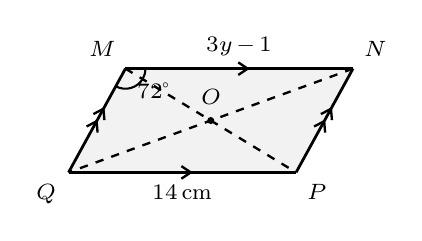
\begin{tikzpicture}[scale=0.85, every node/.style={font=\footnotesize, text=black}]
  \coordinate (Q) at (0,0);
  \coordinate (P) at (3.40,0);
  \coordinate (M) at (0.85,1.55);
  \coordinate (N) at (4.25,1.55);
  \coordinate (O) at ($(M)!0.5!(P)$);
  \fill[gray!10] (M)--(N)--(P)--(Q)--cycle;
  \draw[black, line width=1.0pt, par1] (M)--(N);
  \draw[black, line width=1.0pt, par1] (Q)--(P);
  \draw[black, line width=1.0pt, par2] (Q)--(M);
  \draw[black, line width=1.0pt, par2] (P)--(N);
  \draw[black, line width=0.85pt, dashed] (M)--(P) (N)--(Q);
  \draw[black, line width=0.75pt] ($(M)+(-119:0.30)$) arc (-119:0:0.30);
  \node at (1.28,1.22) {$72^\circ$};
  \fill[black] (O) circle (1.5pt) node[above=2pt] {$O$};
  \node[above left=1pt] at (M) {$M$};
  \node[above right=1pt] at (N) {$N$};
  \node[below right=1pt] at (P) {$P$};
  \node[below left=1pt] at (Q) {$Q$};
  \node[above=1pt] at ($(M)!0.5!(N)$) {$3y-1$};
  \node[below=1pt] at ($(Q)!0.5!(P)$) {$14\unit{cm}$};
\end{tikzpicture}}

\begin{document}
\fontsize{10pt}{15.2pt}\selectfont

% -------------------- ក្បាលកិច្ចតែងការ (Header) --------------------
\begin{center}
  {\muol\fontsize{11pt}{16pt}\selectfont ព្រះរាជាណាចក្រកម្ពុជា}\\[2pt]
  {\muol\fontsize{10pt}{15pt}\selectfont ជាតិ សាសនា ព្រះមហាក្សត្រ}\\[1pt]
  \khmflourish
\end{center}

\vspace{-28pt}
{\muol\fontsize{9.5pt}{12.5pt}\selectfont
មន្ទីរអប់រំ យុវជន និងកីឡា ខេត្តកំពង់ធំ\\
ការិយាល័យអប់រំ យុវជន និងកីឡា ស្រុកកំពង់ស្វាយ\\
អនុវិទ្យាល័យព្រះក្រសាំង}

\vspace{1pt}
\begin{center}
  {\muol\fontsize{10pt}{14pt}\selectfont កិច្ចតែងការបង្រៀន}
\end{center}
\vspace{0pt}

% -------------------- ព័ត៌មានទូទៅ (Metadata) --------------------
{\renewcommand{\arraystretch}{0.95}
\hspace*{4.05cm}%
\begin{tabular}{@{}l l l@{}}
  - \hspace{0.35cm} មុខវិជ្ជា & : & គណិតវិទ្យា ថ្នាក់ទី៨ \\
  - \hspace{0.35cm} ចំណងជើងមេរៀន & : & មេរៀនទី១៣ ចតុកោណ \\
  - \hspace{0.35cm} ចំណងជើងរង & : & ២.១.១ លក្ខណៈប្រលេឡូក្រាម៖ ទ្រឹស្ដីបទទី១--៣ (ទំ.១៧០--១៧១) \\
  - \hspace{0.35cm} រយៈពេល & : & ១ ម៉ោងសិក្សា (៥០ នាទី) \\
  - \hspace{0.35cm} បង្រៀនដោយ & : & ហុក ប៊ុនថែន \\
  - \hspace{0.35cm} កាលបរិច្ឆេទ & : & ថ្ងៃសៅរ៍ ៣កើត ខែមិគសិរ ព.ស.២៥៧០ (១២ ធ្នូ ២០២៦) \\
\end{tabular}

\vspace{1pt}

% -------------------- I. វត្ថុបំណង --------------------
\textbf{I.} {\muol វត្ថុបំណង}\\[1pt]
\hspace*{0.55cm}%
\begin{tabular}{@{}l l L{14.2cm}@{}}
  \wcirc \hspace{0.25cm} វិជ្ជាសម្បទា & : & សិស្សពោលបានត្រឹមត្រូវនូវទ្រឹស្ដីបទទី១ និងវិបាក (អង្កត់ទ្រូងចែកប្រលេឡូក្រាមជាត្រីកោណពីរប៉ុនគ្នា ជ្រុងឈមប៉ុនគ្នាពីរៗ និងមុំឈមប៉ុនគ្នាពីរៗ) ទ្រឹស្ដីបទទី២ (មុំពីរជាប់គ្នាបំពេញគ្នាស្មើ $180^\circ$) និងទ្រឹស្ដីបទទី៣ (អង្កត់ទ្រូងទាំងពីរកាត់គ្នាត្រង់ចំណុចកណ្ដាលនីមួយៗ ដែលជាផ្ចិតឆ្លុះនៃប្រលេឡូក្រាម) តាមសៀវភៅគោល ទំ.១៧០--១៧១ ។ \\
  \wcirc \hspace{0.25cm} បំណិនសម្បទា & : & សិស្សវាស់ពិនិត្យជ្រុង មុំ និងអង្កត់ទ្រូងលើសន្លឹកកិច្ចការស-ខ្មៅ បំពេញតារាងសម្រាយបញ្ជាក់បន្ថយជំនួយតាមលក្ខណៈ \textbf{ម-ជ-ម} គណនារង្វាស់មុំនិងជ្រុងដោយបង្កើតសមីការ និងស្រាយបញ្ជាក់អង្កត់ស្មើគ្នាកាត់តាមផ្ចិតឆ្លុះដោយប្រើសញ្ញា \textbf{[tracing]} និងធនាគារហេតុផល \cnum{1}--\cnum{5} ។ \\
  \wcirc \hspace{0.25cm} ចរិយាសម្បទា & : & សិស្សមានទម្លាប់ផ្ទៀងផ្ទាត់អំណះអំណាងធរណីមាត្រដោយហេតុផលច្បាស់លាស់ (មិនច្រឡំថាអង្កត់ទ្រូងប្រលេឡូក្រាមទូទៅស្មើគ្នាឡើយ) សហការពិភាក្សាជាដៃគូ និងផ្សារភ្ជាប់លក្ខណៈប្រលេឡូក្រាមទៅនឹងគ្រឿងយន្តជន្ទល់កន្ត្រៃក្នុងជីវភាពពិត ។ \\
\end{tabular}

\vspace{1pt}

% -------------------- II. សម្ភារៈឧបទេស --------------------
\textbf{II.} {\muol សម្ភារៈឧបទេស}\\[1pt]
\hspace*{0.55cm}$\bullet$ \hspace{0.35cm} សៀវភៅសិក្សាគោលគណិតវិទ្យាថ្នាក់ទី៨ (ទំ.១៧០--១៧១ និងទំ.១៨៥) ក្ដារខៀន ដីស បន្ទាត់ក្រិត រ៉ាប់ព័រទ័រ ដែកឈាន និងសន្លឹកកិច្ចការសិស្សស-ខ្មៅ (\en{Worksheet\_PARA1} ចំនួន ២ ទំព័រ \en{A4} សម្រាប់វាស់ និងបំពេញផ្ទាល់ ដោយគ្មានស្លាយ \en{LCD}) ។

\vspace{1pt}

% -------------------- III. វិធីសាស្រ្តបង្រៀន --------------------
\textbf{III.} {\muol វិធីសាស្រ្តបង្រៀន}\\[1pt]
\hspace*{0.45cm}%
\begin{tabular}{@{}l l L{14.85cm}@{}}
  $\bullet$ \hspace{0.25cm} គោលវិធី & : & សិស្សមជ្ឈមណ្ឌល (សិក្សាស៊ើបអង្កេតជាដៃគូលើសន្លឹកកិច្ចការបំពេញផ្ទាល់ គ្មានស្លាយ \en{LCD}) \\
  $\bullet$ \hspace{0.25cm} យុទ្ធវិធីបង្រៀន & : & គម្រូស្ថាបនានិយម \en{5Es} រួមបញ្ចូល \textbf{ការបំបែកតាមអង្កត់ទ្រូងជំនួយ និងតារាងសម្រាយបញ្ជាក់បន្ថយជំនួយជាជំហាន} (\en{Faded Proof Scaffolding — Miyazaki et al., 2017; Anwar et al., 2023}) \\
\end{tabular}
}

\vspace{1pt}

% -------------------- IV. ដំណើរការបង្រៀន --------------------
\textbf{IV.} {\muol ដំណើរការបង្រៀន}

\vspace{1pt}

\renewcommand{\arraystretch}{1.15}
\begin{longtable}{|L{5.50cm}|L{7.90cm}|L{4.80cm}|}
\hline
\rowcolor{headgray}
\multicolumn{1}{|c|}{\muol សកម្មភាពគ្រូ} &
\multicolumn{1}{c|}{\muol ខ្លឹមសារមេរៀន} &
\multicolumn{1}{c|}{\muol សកម្មភាពសិស្ស} \\
\hline
\endfirsthead
\hline
\endhead
\hline
\endfoot
\hline
\endlastfoot

% ==================== ជំហានទី១ (2min) ====================
\stepheader{ជំហានទី១ \enbf{(}រដ្ឋបាលថ្នាក់\enbf{)}}
$\bullet$ ពិនិត្យអវត្តមាន សណ្ដាប់ធ្នាប់ អនាម័យ និងសម្ភារៈធរណីមាត្រ (បន្ទាត់ក្រិត និងរ៉ាប់ព័រទ័រ)
&
$\bullet$ ពិនិត្យវត្តមាន និងសណ្ដាប់ធ្នាប់ថ្នាក់រៀន \par
$\bullet$ ត្រៀមបន្ទាត់ក្រិត និងរ៉ាប់ព័រទ័រសម្រាប់វាស់លើសន្លឹកកិច្ចការ
&
$\circ$ ប្រធានថ្នាក់រាយការណ៍អវត្តមាន និងត្រៀមឧបករណ៍ធរណីមាត្រ \\[3pt]

$\bullet$ រៀបចំសិស្សជាដៃគូពិភាក្សា រួចចែកសន្លឹកកិច្ចការ \en{Worksheet\_PARA1} (២ ទំព័រ \en{A4}) ផ្កាប់លើតុ
&
$\bullet$ ការចាត់ដៃគូសិក្សា និងចែកសន្លឹកកិច្ចការស-ខ្មៅ
&
$\circ$ អង្គុយតាមដៃគូ និងទទួលសន្លឹកកិច្ចការទុកលើតុ \\
\hline

% ==================== ជំហានទី២ (9min: <=3 + 3 + E1 3) ====================
\stepheader{ជំហានទី២ \enbf{(}កិច្ចការផ្ទះ \enbf{+} ទំនាក់ទំនងមេរៀនថ្មី\enbf{)}}
\ditem \textbf{កំណែកិច្ចការផ្ទះ ($\le 3\unit{min}$)} \timenote{សង្ខេបខ្លីលើក្ដារខៀន}
&
{\centering\redsub{កំណែកិច្ចការផ្ទះ (លំហាត់ទី៦ ក ទំ.១៨៥)}\par}
&
$\circ$ យកសៀវភៅកិច្ចការផ្ទះមកផ្ទៀងផ្ទាត់ \\[2pt]

$\bullet$ ហៅសិស្ស ១ រូបបញ្ជាក់ហេតុផលលើរូបប្រលេឡូក្រាម $ABCD$ ($\ang{A}=60^\circ, AB=6\unit{cm}, AD=4\unit{cm}$)
&
$\bullet$ ដោយ $\ang{A}=60^\circ \neq 90^\circ$ វា\textbf{មិនមែនជាចតុកោណកែង}ទេ ហើយដោយជ្រុងជាប់ $AB=6\unit{cm}\neq AD=4\unit{cm}$ វា\textbf{មិនមែនជាចតុកោណស្មើ}ទេ ។
&
$\circ$ ផ្ទៀងផ្ទាត់ចម្លើយ និងកែលម្អចំណុចខ្វះខាត \\[3pt]

\ditem \textbf{រំលឹកមេរៀនទាក់ទង ($3\unit{min}$)} \par
$\bullet$ គូសរូបលើក្ដារខៀន សួររំលឹកទី១៖ បើ $AB \parallel DC$ កាត់ដោយ $AC$ តើមុំឆ្លាស់ក្នុង និងមុំក្នុងរួមខាងមានទំនាក់ទំនងដូចម្ដេច?
&
{\centering\redsub{រំលឹកមេរៀនទាក់ទងមេរៀនថ្មី}\par} \par
$\bullet$ បើ $AB \parallel DC$៖ មុំឆ្លាស់ក្នុងស្មើគ្នា ($\ang{BAC}=\ang{DCA}$) រីឯមុំក្នុងរួមខាងបំពេញគ្នា ($\ang{BAD}+\ang{ADC}=180^\circ$) ។
&
$\circ$ សង្កេតរូបលើក្ដារខៀន និងឆ្លើយ៖ «មុំឆ្លាស់ក្នុងស្មើគ្នា រីឯមុំក្នុងរួមខាងបូកចូលគ្នាស្មើ $180^\circ$» \\[2pt]

– \textbf{សំណួរទី២៖} តើលក្ខណៈត្រីកោណប៉ុនគ្នា \textbf{ម-ជ-ម} ត្រូវការធាតុអ្វីខ្លះ?
&
$\bullet$ លក្ខណៈ \textbf{ម-ជ-ម}៖ ជ្រុងមួយស្មើគ្នា និងមុំពីរជាប់ជ្រុងនោះស្មើគ្នារៀងគ្នា ។
&
$\circ$ រំលឹកលក្ខណៈត្រីកោណប៉ុនគ្នា \textbf{ម-ជ-ម} \\[3pt]

&
\cfig{\figPrereqPARA}
& \\[3pt]

\fiveE{E1 - Engage (3min)} \timenote{(កុំទាន់ផ្ដល់ចម្លើយ)} \par
\ditem \textbf{បញ្ហាភ្ញាក់ផ្អើល «ជន្ទល់កន្ត្រៃលើកទំនិញរាងប្រលេឡូក្រាម»៖} \par
$\bullet$ គូសរូបស៊ុមជន្ទល់កន្ត្រៃ $ABCD$ ($AB\parallel DC, AD\parallel BC$) ភ្ជាប់ដែកទ្រូង $AC$ និង $BD$ ត្រង់ប៊ូឡុង $O$
&
{\centering\redsub{ស្ថានភាពបញ្ហា៖ យានដ្ឋានជួសជុលរថយន្តកំពង់ស្វាយ}\par}
&
$\circ$ សង្កេតរូបជន្ទល់កន្ត្រៃលើក្ដារខៀន និងលើក្បាលសន្លឹកកិច្ចការ \\[3pt]

&
\cfig{\figEngagePARA}
& \\[3pt]

– \textbf{សំណួរបំផុសទី១៖} «កូនជាង ក អះអាងថា ក្នុងប្រលេឡូក្រាម $ABCD$ ជ្រុងឈមស្មើគ្នា ហើយដែកទ្រូងទាំងពីរក៏ស្មើគ្នាដែរ ($AC=BD$)!»
&
\textbf{ចម្ងល់គោលប្រចាំម៉ោង៖} \par
(១) តើជ្រុងឈម និងមុំឈមនៃប្រលេឡូក្រាមមានទំនាក់ទំនងដូចម្ដេច?
&
$\circ$ ស្ដាប់ស្ថានភាពបញ្ហារវាងកូនជាង ក និងកូនជាង ខ \\[2pt]

– \textbf{សំណួរបំផុសទី២៖} «រីឯកូនជាង ខ ថា $AC\neq BD$ ប៉ុន្តែប៊ូឡុង $O$ ចែកដែកទ្រូងនីមួយៗជាពីរស្មើគ្នា ($OA=OC, OB=OD$)! តើដៃគូអ្នកគាំទ្រនរណា?»
&
(២) តើអង្កត់ទ្រូងប្រលេឡូក្រាមទូទៅស្មើគ្នា ($AC=BD$) ឬគ្រាន់តែកាត់គ្នាត្រង់ចំណុចកណ្ដាលនីមួយៗ?
&
$\circ$ ពិភាក្សាជាដៃគូ ៣០ វិនាទី រួចគូសធីកការទស្សន៍ទាយដំបូងក្នុងប្រអប់ \en{E1} លើសន្លឹកកិច្ចការ \\
\hline

% ==================== ជំហានទី៣ (17min: E2 11m + E3 6m) ====================
\stepheader{ជំហានទី៣ \enbf{(}ខ្លឹមសារមេរៀនថ្មី\enbf{)}}
\fiveE{E2 - Explore (11min)} \par
$\bullet$ សរសេរចំណងជើងរងលើក្ដារខៀន និងឱ្យសិស្សបើកសន្លឹកកិច្ចការទំព័រទី១ ផ្នែកទី២
&
២. លក្ខណៈចតុកោណពិសេស \par
២.១ លក្ខណៈប្រលេឡូក្រាម៖ ទ្រឹស្ដីបទទី១--៣ (ទំ.១៧០--១៧១)
&
$\circ$ កត់ចំណងជើងរងចូលសៀវភៅសរសេរ និងត្រៀមបន្ទាត់ក្រិត-រ៉ាប់ព័រទ័រ \\[3pt]

\ditem \textbf{សកម្មភាពទី១៖ ពិសោធន៍វាស់ខ្នាតពិត និងអន្ទាក់អង្កត់ទ្រូង ($5.5\unit{min}$)} \par
$\bullet$ ឱ្យដៃគូសិស្សវាស់ប្រលេឡូក្រាមខ្នាតពិត $ABCD$ លើសន្លឹកកិច្ចការ ($AB=5.0\unit{cm}, AD=3.2\unit{cm}, \ang{D}=60^\circ$)
&
{\centering\textbf{លទ្ធផលពិសោធន៍វាស់ និង \en{POE} អន្ទាក់អង្កត់ទ្រូង}\par} \par
$\bullet$ ជ្រុងឈម៖ $AB=DC=5.0\unit{cm}$, $AD=BC=3.2\unit{cm}$ ។ \par
$\bullet$ មុំឈម និងមុំជាប់៖ $\ang{D}=\ang{B}=60^\circ$, $\ang{A}=\ang{C}=120^\circ$ ($\ang{A}+\ang{B}=180^\circ$) ។
&
$\circ$ វាស់ប្រវែងជ្រុងទាំង ៤ និងមុំទាំង ៤ ជាក់ស្ដែងលើសន្លឹកកិច្ចការ \\[2pt]

$\bullet$ ឱ្យសិស្សវាស់អង្កត់ទ្រូង $AC, BD$ និងកំណាត់ $OA, OC, OB, OD$ ដើម្បីផ្ទៀងផ្ទាត់ការទស្សន៍ទាយ \en{E1}!
&
$\bullet$ \textbf{បំបែកការយល់ច្រឡំ (\en{POE})៖} $AC\approx 7.2\unit{cm} \neq BD\approx 4.4\unit{cm}$ (\graybox{អង្កត់ទ្រូងមិនស្មើគ្នាទេ!}) ប៉ុន្តែ $OA=OC\approx 3.6\unit{cm}$ និង $OB=OD\approx 2.2\unit{cm}$!
&
$\circ$ ភ្ញាក់ផ្អើលពេលឃើញ $AC\neq BD$ ប៉ុន្តែ $OA=OC$ និង $OB=OD$ \\[3pt]

\ditem \textbf{សកម្មភាពទី២៖ តារាងសម្រាយបញ្ជាក់បន្ថយជំនួយ ($5.5\unit{min}$)} \par
$\bullet$ ណែនាំឱ្យសិស្សគូស \textbf{[tracing]} ព័ទ្ធរង្វង់ជ្រុងរួម $AC$ និងធ្នូមុំឆ្លាស់ក្នុង ដើម្បីបំពេញ \textbf{ផ្នែក ក} ($\tri{ADC}$ និង $\tri{ABC}$)
&
\textbf{គោលគំនិតសម្រាយបញ្ជាក់តាមអង្កត់ទ្រូងជំនួយ៖} \par
$\bullet$ \textbf{ផ្នែក ក (ទ្រឹស្ដីបទទី១--២)៖} ក្នុង $\tri{ADC}$ និង $\tri{ABC}$ មាន៖ \par
$\ang{DAC}=\ang{BCA}$ (ឆ្លាស់ក្នុង $AD\parallel BC$), $AC$ ជ្រុងរួម, $\ang{DCA}=\ang{BAC}$ (ឆ្លាស់ក្នុង $AB\parallel DC$) $\Rightarrow \tri{ADC}\cg\tri{ABC}$ (\textbf{ម-ជ-ម}) ។
&
$\circ$ គូសសញ្ញា \textbf{[tracing]} លើរូបទី១ និងបំពេញតារាងសម្រាយបញ្ជាក់ \textbf{ផ្នែក ក} ជាដៃគូ \\[2pt]

$\bullet$ ណែនាំឱ្យបន្តគូសសញ្ញាឆ្នូតលើ $AB=DC$ និងធ្នូមុំឆ្លាស់ក្នុង ដើម្បីបំពេញ \textbf{ផ្នែក ខ} ($\tri{AOB}$ និង $\tri{COD}$)
&
$\bullet$ \textbf{ផ្នែក ខ (ទ្រឹស្ដីបទទី៣)៖} ក្នុង $\tri{AOB}$ និង $\tri{COD}$ មាន៖ \par
$\ang{OAB}=\ang{OCD}$, $AB=DC$, $\ang{OBA}=\ang{ODC}$ $\Rightarrow \tri{AOB}\cg\tri{COD}$ (\textbf{ម-ជ-ម}) $\Rightarrow OA=OC$ និង $OB=OD$ ។
&
$\circ$ បំពេញតារាងសម្រាយបញ្ជាក់ \textbf{ផ្នែក ខ} រហូតទាញបាន $OA=OC, OB=OD$ \\[3pt]

\fiveE{E3 - Explain (6min)} \par
\ditem \textbf{បង្គុំទ្រឹស្ដីបទទី១ ដល់ទី៣ និងធនាគារហេតុផល \cnum{1}--\cnum{5}៖} \par
$\bullet$ ហៅតំណាងដៃគូ ២ ក្រុមឡើងបំពេញជំហានសម្រាយបញ្ជាក់លើក្ដារខៀន
&
\textbf{សង្ខេបទ្រឹស្ដីបទ និងធនាគារហេតុផល \cnum{1}--\cnum{5}៖} \par
\cnum{1} \textbf{និយមន័យប្រលេឡូក្រាម៖} ជ្រុងឈមស្របគ្នាពីរៗ ($AB\parallel DC, AD\parallel BC$) ។ \par
\cnum{2} \textbf{ទ្រឹស្ដីបទទី១៖} អង្កត់ទ្រូងនីមួយៗនៃប្រលេឡូក្រាមចែកប្រលេឡូក្រាមជាត្រីកោណពីរប៉ុនគ្នា ($\tri{ADC}\cg\tri{ABC}$) ។
&
$\circ$ តំណាងដៃគូឡើងបកស្រាយ និងសិស្សបំពេញ \cnum{1}--\cnum{2} លើសន្លឹកកិច្ចការទំព័រទី២ \\[2pt]

$\bullet$ គ្រូសង្ខេបវិបាកនៃទ្រឹស្ដីបទទី១ តាមសៀវភៅគោល ទំ.១៧០
&
\cnum{3} \textbf{វិបាកទ្រឹស្ដីបទទី១៖} ក្នុងប្រលេឡូក្រាម \textbf{ជ្រុងឈមប៉ុនគ្នាពីរៗ} ($AB=DC, AD=BC$) និង\textbf{មុំឈមប៉ុនគ្នាពីរៗ} ($\ang{A}=\ang{C}, \ang{B}=\ang{D}$) ។
&
$\circ$ បំពេញវិបាក \cnum{3} ចូលក្នុងប្រអប់ធនាគារហេតុផល \\[3pt]

&
\cfig{\figTheoremsPARA}
& \\[3pt]

$\bullet$ សង្កត់ធ្ងន់លើទ្រឹស្ដីបទទី២ និងលក្ខណៈ \textbf{ផ្ចិតឆ្លុះ $O$} ក្នុងទ្រឹស្ដីបទទី៣
&
\cnum{4} \textbf{ទ្រឹស្ដីបទទី២៖} មុំពីរជាប់គ្នានៃប្រលេឡូក្រាមជាមុំបំពេញគ្នា ($\ang{A}+\ang{B}=180^\circ$) ។ \par
\cnum{5} \textbf{ទ្រឹស្ដីបទទី៣៖} អង្កត់ទ្រូងទាំងពីរនៃប្រលេឡូក្រាមកាត់គ្នាត្រង់ចំណុចកណ្ដាលនីមួយៗ ($OA=OC, OB=OD$) ។ ចំណុចប្រសព្វ $O$ ហៅថា \textbf{ផ្ចិតឆ្លុះនៃប្រលេឡូក្រាម} ។
&
$\circ$ កត់ត្រា \cnum{4}--\cnum{5} និងកត់សម្គាល់អត្ថន័យនៃផ្ចិតឆ្លុះ $O$ \\
\hline

% ==================== ជំហានទី៤ (20min: E4 10m + E5 10m) ====================
\stepheader{ជំហានទី៤ \enbf{(}ពង្រឹង និងពង្រីកចំណេះដឹង\enbf{)}}
\fiveE{E4 - Elaborate (10min)} \par
\ditem \textbf{លំហាត់គំរូអនុវត្តចេញពីសៀវភៅគោល (ទំ.១៨៥ លំហាត់ទី៤ និងទី២)៖} \par
$\bullet$ ដឹកនាំសិស្សអាន និងវិភាគប្រធានលំហាត់គំរូទី១ លើសន្លឹកកិច្ចការទំព័រទី២
&
{\muol លំហាត់គំរូទី១} \textbf{(លំហាត់ទី៤ ទំ.១៨៥ — គណនាមុំតាមសមីការ)៖} \par
គណនារង្វាស់មុំទាំងបួននៃប្រលេឡូក្រាម $ABCD$ ដោយដឹងថារង្វាស់មុំមួយស្មើពីរដងនៃរង្វាស់មុំមួយទៀត ។
&
$\circ$ អានប្រធានគំរូទី១ និងកំណត់ទំនាក់ទំនងរវាងមុំទាំងពីរ \\[2pt]

$\bullet$ ដឹកនាំសិស្សអានប្រធានគំរូទី២ និងគូសសញ្ញា \textbf{[tracing]} ជុំវិញផ្ចិត $I$
&
{\muol លំហាត់គំរូទី២} \textbf{(លំហាត់ទី២ ទំ.១៨៥ — អង្កត់កាត់តាមផ្ចិតឆ្លុះ)៖} \par
ប្រលេឡូក្រាម $ABCD$ មានផ្ចិត $I$ ។ បន្ទាត់ $d$ កាត់តាម $I$ ជួប $AB$ ត្រង់ $E$ និង $CD$ ត្រង់ $F$ ។ ចូរស្រាយបញ្ជាក់ថា $IE = IF$ ។
&
$\circ$ គូសសញ្ញា \textbf{[tracing]} លើរូបគំរូទី២ ក្នុងសន្លឹកកិច្ចការទំព័រទី២ \\[3pt]

&
\cfig{\figModelPARA}
& \\[3pt]

$\bullet$ សួរបំផុសគំរូទី១៖ «ហេតុអ្វីមុំដែលស្មើ $2$ ដងនៃមុំមួយទៀត មិនអាចជាមុំឈមគ្នាទេ តែត្រូវតែជាមុំជាប់គ្នា?»
&
\textbf{ដំណោះស្រាយសង្ខេប៖} \par
$\bullet$ \textbf{គំរូទី១៖} ព្រោះមុំឈមស្មើគ្នា (\cnum{3}) ដូច្នេះមុំទាំងពីរជាមុំជាប់គ្នា៖ តាង $\ang{A}=x \Rightarrow \ang{B}=2x$ ។ តាម \cnum{4}៖ $x+2x=180^\circ \Rightarrow 3x=180^\circ \Rightarrow x=60^\circ$ ។ \par
ដូច្នេះ $\ang{A}=\ang{C}=60^\circ$ និង $\ang{B}=\ang{D}=120^\circ$ ។
&
$\circ$ បង្កើតសមីការ $x+2x=180^\circ$ និងគណនាមុំទាំងបួនលើសន្លឹកកិច្ចការ \\[2pt]

$\bullet$ សួរបំផុសគំរូទី២៖ «តើផ្ចិត $I$ ផ្ដល់អង្កត់ណាខ្លះស្មើគ្នាតាម \cnum{5}?»
&
$\bullet$ \textbf{គំរូទី២៖} ក្នុង $\tri{IAE}$ និង $\tri{ICF}$ មាន៖ \par
(១) $\ang{IAE}=\ang{ICF}$ (ឆ្លាស់ក្នុង $AB\parallel CD$, \cnum{1}); (២) $IA=IC$ (ផ្ចិត $I$, \cnum{5}); (៣) $\ang{AIE}=\ang{CIF}$ (ទល់កំពូល) $\Rightarrow \tri{IAE}\cg\tri{ICF}$ (\textbf{ម-ជ-ម}) $\Rightarrow$ \graybox{$IE=IF$} ។
&
$\circ$ បំពេញសម្រាយបញ្ជាក់គំរូទី២ ដោយភ្ជាប់ហេតុផល \cnum{1} និង \cnum{5} \\[2pt]

– \textbf{សំណួរឆ្លុះបញ្ចាំង (\en{EIA Looking-Back})៖} «ហេតុអ្វីយើងជ្រើសផ្គូផ្គង $\tri{IAE}$ និង $\tri{ICF}$ ដែលមានកំពូលរួមត្រង់ផ្ចិត $I$?»
&
$\bullet$ \textbf{គន្លឹះវិភាគ៖} ព្រោះរាល់បន្ទាត់កាត់តាមផ្ចិតឆ្លុះ $I$ ភ្ជាប់ជាមួយអង្កត់ទ្រូង $AC$ បង្កើតបានគូជ្រុងស្មើ $IA=IC$ និងមុំទល់កំពូលស្មើគ្នាភ្លាមៗ!
&
$\circ$ កត់សម្គាល់យុទ្ធសាស្ត្រជ្រើសត្រីកោណជុំវិញផ្ចិតឆ្លុះ $I$ \\[3pt]

\fiveE{E5 - Evaluate (10min)} \par
\ditem \textbf{លំហាត់ប្រតិបត្តិ និងផ្ទៀងផ្ទាត់ជាដៃគូ ($6.5\unit{min}$, ផ្នែកទី៥)៖} \par
$\bullet$ ឱ្យសិស្សធ្វើលំហាត់ប្រតិបត្តិដោយឯករាជ្យ ៤ នាទី លើសន្លឹកកិច្ចការ
&
{\muol លំហាត់ប្រតិបត្តិ} \textbf{(គណនាជ្រុង មុំ និងអង្កត់ទ្រូង)៖} \par
ប្រលេឡូក្រាម $MNPQ$ មានផ្ចិត $O$, $MN=3y-1\unit{cm}$, $QP=14\unit{cm}$, $MO=4.5\unit{cm}$ និង $\ang{M}=72^\circ$ ។
&
$\circ$ អានប្រធាន និងពិនិត្យធាតុស្គាល់លើរូបប្រលេឡូក្រាម $MNPQ$ \\[3pt]

&
\cfig{\figPractPARA}
& \\[3pt]

$\bullet$ ឱ្យសិស្សប្ដូរសន្លឹកកិច្ចការផ្ទៀងជាមួយដៃគូ (\en{Peer-Check}) ២.៥ នាទី និងឆ្លើយបិទបញ្ហាជន្ទល់កន្ត្រៃ \en{E1}
&
១. តាម \cnum{3}៖ $3y-1=14 \Rightarrow 3y=15 \Rightarrow$ \graybox{$y=5\unit{cm}$} ។ \par
២. តាម \cnum{3} និង \cnum{4}៖ $\ang{P}=72^\circ$, $\ang{N}=\ang{Q}=180^\circ-72^\circ=$ \graybox{$108^\circ$} ។ \par
៣. តាម \cnum{5}៖ អង្កត់ទ្រូង $MP = 2\times MO =$ \graybox{$9\unit{cm}$} ។ \par
$\bullet$ \textbf{បិទបញ្ហា E1៖} កូនជាង ខ ត្រឹមត្រូវ! $AC\neq BD$ តែ $OA=OC, OB=OD$ ។
&
$\circ$ គណនាចម្លើយ ប្ដូរផ្ទៀងជាមួយដៃគូ និងសរសេរចម្លើយបិទបញ្ហា \en{E1} \\[3pt]

\ditem \textbf{សំណួរត្រួតពិនិត្យរហ័ស \en{Exit Check A--D} ($3.5\unit{min}$)៖} \par
$\bullet$ ឱ្យសិស្សគូសរង្វង់ចម្លើយត្រឹមត្រូវក្នុងប្រអប់ \en{Exit Check} លើសន្លឹកកិច្ចការ រួចលើកម្រាមដៃ ១--៤ បង្ហាញចម្លើយ
&
\textbf{សំណួរ Exit Check (អន្ទាក់មុំជាប់ ទល់នឹង មុំឈម)៖} \par
«ក្នុងប្រលេឡូក្រាម $ABCD$ បើ $\ang{A}=3x+10^\circ$ និង $\ang{B}=2x-5^\circ$ តើតម្លៃ $x$ ស្មើប៉ុន្មាន?» \par
\en{A.} $x=15^\circ$ \quad \graybox{\enbf{B.} $x=35^\circ$ \ding{51}} \quad \en{C.} $x=37^\circ$ \quad \en{D.} $x=70^\circ$ \par
{\footnotesize (ព្រោះ $(3x+10^\circ)+(2x-5^\circ)=180^\circ \Rightarrow 5x+5^\circ=180^\circ \Rightarrow x=35^\circ$)}
&
$\circ$ គូសរង្វង់ជ្រើសរើស \textbf{B} លើសន្លឹកកិច្ចការ និងលើកម្រាមដៃ ២ ផ្ទៀងផ្ទាត់ជាមួយគ្រូ \\
\hline

% ==================== ជំហានទី៥ (<=2min) ====================
\stepheader{ជំហានទី៥ \enbf{(}កិច្ចការផ្ទះ \enbf{+} បណ្ដាំផ្ញើ\enbf{)}}
$\bullet$ កត់ត្រាកិច្ចការផ្ទះលើក្ដារខៀន (មានបោះពុម្ពស្រាប់នៅផ្នែកទី៦ នៃសន្លឹកកិច្ចការទំព័រទី២)
&
{\centering{\muol កិច្ចការផ្ទះ} \textbf{(សៀវភៅគោល ទំព័រ ១៨៥)}\par} \par
១. \textbf{លំហាត់ទី៥ ទំ.១៨៥៖} បើមុំមួយនៃប្រលេឡូក្រាមស្មើ $(2x+20^\circ)$ ហើយមុំតគ្នាមួយទៀតស្មើ $(x-50^\circ)$ ចូរគណនាតម្លៃ $x$ និងមុំទាំងបួន ។ \par
២. \textbf{លំហាត់ទី៧ ទំ.១៨៥ (ផ្នែកទី១)៖} ប្រលេឡូក្រាម $ABCD$ មានផ្ចិត $O$ ។ បន្ទាត់ $d$ កាត់តាម $O$ ជួប $AB, CD$ ត្រង់ $A', C'$ និងបន្ទាត់ $\Delta$ កាត់តាម $O$ ជួប $BC, AD$ ត្រង់ $B', D'$ ។ ចូរបង្ហាញថា $OA'=OC'$ និង $OB'=OD'$ ។
&
$\circ$ កត់ត្រាកិច្ចការផ្ទះ និងទុកដាក់សន្លឹកកិច្ចការក្នុងសៀវភៅសរសេរ \\[3pt]

$\bullet$ ណែនាំឱ្យអានមេរៀនបន្ទាប់ជាមុន និងផ្ដាំផ្ញើវិន័យសិក្សា
&
$\bullet$ \textbf{អានជាមុន៖} ២.១ លក្ខណៈសម្គាល់ប្រលេឡូក្រាម (ទ្រឹស្ដីបទទី៤--៧ ទំព័រ ១៧១--១៧៤) \par
$\bullet$ បណ្ដាំផ្ញើ៖ ធ្វើកិច្ចការផ្ទះឱ្យទៀងទាត់ និងជួយការងារគ្រួសារ ។
&
$\circ$ ទទួលបណ្ដាំផ្ញើ និងជម្រាបលាគ្រូ \\
\end{longtable}

% -------------------- កាលបរិច្ឆេទ និងហត្ថលេខា (Date & Signature) --------------------
\vspace{16pt}
\hfill
\begin{minipage}{9.8cm}
  {\centering
    ថ្ងៃសៅរ៍ ៣កើត ខែមិគសិរ ឆ្នាំមមី អដ្ឋស័ក ពុទ្ធសករាជ ២៥៧០\\[3pt]
    កំពង់ស្វាយ, ថ្ងៃទី១២ ខែធ្នូ ឆ្នាំ២០២៦\\[4pt]
    {\muol គ្រូបង្រៀន}\par}
  \vspace{34pt}
  \hfill{\muol ហុក ប៊ុនថែន}\hspace*{1.4cm}
\end{minipage}

\end{document}
